\begin{figure}
  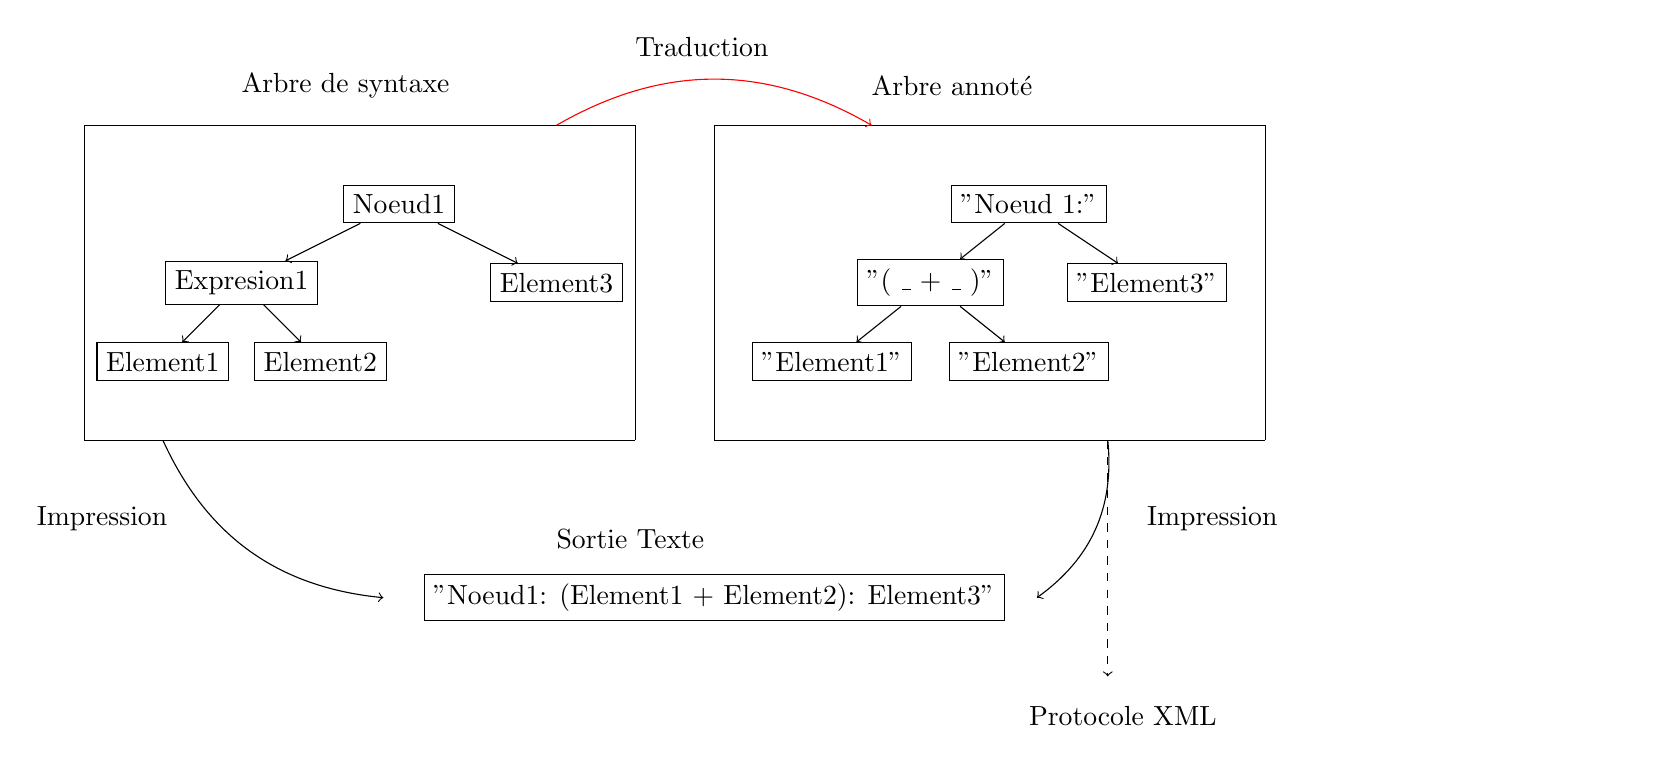
\begin{tikzpicture}
    %% Rectangle
    \draw (-5,-3) -- (-5,1);
    \draw (-5,-3) -- (2,-3);
    \draw (2,1) -- (-5,1);
    \draw (2,1) -- (2,-3);

    %% graphe1
    \node[text width=6cm] (titre1) at (0,1.5) {Arbre de syntaxe};
    \node[draw] (Noeud1) at (-1,0) {Noeud1};
    \node[draw] (Expression1) at (-3,-1) {Expresion1};
    \node[draw] (Element3) at (1,-1) {Element3};
    \node[draw] (Element1) at (-4,-2) {Element1};
    \node[draw] (Element2) at (-2,-2) {Element2};
    \draw[->] (Noeud1) -> (Expression1);
    \draw[->] (Noeud1) -> (Element3);
    \draw[->] (Expression1) -> (Element1);
    \draw[->] (Expression1) -> (Element2);

    % Rectangle 2
    \draw (3,-3) -- (3,1);
    \draw (3,-3) -- (10,-3);
    \draw (10,1) -- (3,1);
    \draw (10,1) -- (10,-3);

    % graphe2
    \node[text width=6cm] (titre2) at (8,1.5) {Arbre annoté};
    \node[draw] (INoeud1)      at (7,0) {"Noeud 1:"};
    \node[draw] (IExpression1) at (5.75,-1) {"( \_ + \_ )"};
    \node[draw] (IElement3)    at (8.5,-1) {"Element3"};
    \node[draw] (IElement1)    at (4.5,-2) {"Element1"};
    \node[draw] (IElement2)    at (7,-2) {"Element2"};
    \draw[->] (INoeud1) -> (IExpression1);
    \draw[->] (INoeud1) -> (IElement3);
    \draw[->] (IExpression1) -> (IElement1);
    \draw[->] (IExpression1) -> (IElement2);

    %%graph3
    \node[text width=6cm] (titre3) at (4,-4.25) {Sortie Texte};
    \node[draw] (Pp) at (3,-5) {"Noeud1: (Element1 + Element2): Element3"};

   \node[text width=6cm] (lab1) at (-2.6, -4) {Impression};
   \draw[->] (-4,-3) to [bend right] (-1.2,-5);
   \node[text width=6cm] (lab2) at (11.5, -4) {Impression};
   \draw[->] (8,-3) to [bend left] (7.1,-5);

   \node[text width=6cm] (lab3) at (5, 2) {Traduction};
   \draw[->,red] (1,1) to [bend left] (5,1);

   \draw[->, dashed] (8,-3) to (8, -6);
   \node[text width=6cm] (xml1) at (10,-6.5) {Protocole XML};
  \end{tikzpicture}
  \caption{Traduction de l'arbre de syntaxe abstraite\label{trad1}}
\end{figure}
